% =====================================================================
% 6. Final comparison and discussion (PRDL, Maria Martinez)
% T15 (shared); published results from report/published.json (chat DL 09).
% =====================================================================
\section{Final comparison and discussion}\label{sec:discussion}

\subsection{All final models on the test fold}

Table~\ref{tab:comparison_final} and Figure~\ref{fig:comparison_overview} gather every final model of the
project on the test fold: the trivial model, the five families with 12 leads, the same five on lead II,
the six transfer configurations of the ECG-GPT and zero-shot CLIP. Table~\ref{tab:comparison_per_class}
gives the AUROC per superclass. With 12 leads, HYP is the hardest class for the CNN and the recurrent
models and CD for the Transformer, and the ranking of the families with 12 leads is the same as in Section~\ref{sec:arch-summary}.

% Shared float (common/make_floats.py). Table: tables/comparison_final.tex
\begin{table}[htbp]
\centering
\caption[Final comparison (test)]{Final comparison on the test fold. Mean $\pm$ SD over seeds; interval: 95\,\% patient bootstrap of the first seed. Published rows: macro AUC of the superclass task in Table~I of \cite{strodthoff2021deep}, obtained in a different setting (described in the text).}
\label{tab:comparison_final}
\small
\begin{adjustbox}{max width=\textwidth}
% Generated by src/comparison.py from results/logs/comparison_summary.json.
% Mean +- SD over seeds (one run: no SD); CI = 95% patient bootstrap of the first seed. Needs alias "comparison".
\begin{tabular}{lcrrccc}
\toprule
Model & Labels & Train.\ param. & Seeds & Test macro AUROC & First seed [95\% CI] & Test macro F1 \\
\midrule
\multicolumn{7}{l}{\textit{12 leads}} \\
\quad Trivial (lead mean and SD) & 100\% & \comparisonParamsTrivial{} & \comparisonNSeedsTrivial{} & \comparisonTestAurocMeanTrivial{} & \comparisonTestAurocFirstTrivial{} [\comparisonTestAurocLoFirstTrivial{}, \comparisonTestAurocHiFirstTrivial{}] & \comparisonTestFOneMeanTrivial{} \\
\quad Dense & 100\% & \comparisonParamsTwelveDense{} & \comparisonNSeedsTwelveDense{} & \comparisonTestAurocMeanTwelveDense{} $\pm$ \comparisonTestAurocSdTwelveDense{} & \comparisonTestAurocFirstTwelveDense{} [\comparisonTestAurocLoFirstTwelveDense{}, \comparisonTestAurocHiFirstTwelveDense{}] & \comparisonTestFOneMeanTwelveDense{} $\pm$ \comparisonTestFOneSdTwelveDense{} \\
\quad CNN & 100\% & \comparisonParamsTwelveCnn{} & \comparisonNSeedsTwelveCnn{} & \comparisonTestAurocMeanTwelveCnn{} $\pm$ \comparisonTestAurocSdTwelveCnn{} & \comparisonTestAurocFirstTwelveCnn{} [\comparisonTestAurocLoFirstTwelveCnn{}, \comparisonTestAurocHiFirstTwelveCnn{}] & \comparisonTestFOneMeanTwelveCnn{} $\pm$ \comparisonTestFOneSdTwelveCnn{} \\
\quad RNN & 100\% & \comparisonParamsTwelveRnn{} & \comparisonNSeedsTwelveRnn{} & \comparisonTestAurocMeanTwelveRnn{} $\pm$ \comparisonTestAurocSdTwelveRnn{} & \comparisonTestAurocFirstTwelveRnn{} [\comparisonTestAurocLoFirstTwelveRnn{}, \comparisonTestAurocHiFirstTwelveRnn{}] & \comparisonTestFOneMeanTwelveRnn{} $\pm$ \comparisonTestFOneSdTwelveRnn{} \\
\quad RNN + attention & 100\% & \comparisonParamsTwelveRnnattn{} & \comparisonNSeedsTwelveRnnattn{} & \comparisonTestAurocMeanTwelveRnnattn{} $\pm$ \comparisonTestAurocSdTwelveRnnattn{} & \comparisonTestAurocFirstTwelveRnnattn{} [\comparisonTestAurocLoFirstTwelveRnnattn{}, \comparisonTestAurocHiFirstTwelveRnnattn{}] & \comparisonTestFOneMeanTwelveRnnattn{} $\pm$ \comparisonTestFOneSdTwelveRnnattn{} \\
\quad Transformer & 100\% & \comparisonParamsTwelveTransformer{} & \comparisonNSeedsTwelveTransformer{} & \comparisonTestAurocMeanTwelveTransformer{} $\pm$ \comparisonTestAurocSdTwelveTransformer{} & \comparisonTestAurocFirstTwelveTransformer{} [\comparisonTestAurocLoFirstTwelveTransformer{}, \comparisonTestAurocHiFirstTwelveTransformer{}] & \comparisonTestFOneMeanTwelveTransformer{} $\pm$ \comparisonTestFOneSdTwelveTransformer{} \\
\addlinespace
\multicolumn{7}{l}{\textit{Lead II only (T14)}} \\
\quad Dense & 100\% & \comparisonParamsOneleadDense{} & \comparisonNSeedsOneleadDense{} & \comparisonTestAurocMeanOneleadDense{} $\pm$ \comparisonTestAurocSdOneleadDense{} & \comparisonTestAurocFirstOneleadDense{} [\comparisonTestAurocLoFirstOneleadDense{}, \comparisonTestAurocHiFirstOneleadDense{}] & \comparisonTestFOneMeanOneleadDense{} $\pm$ \comparisonTestFOneSdOneleadDense{} \\
\quad CNN & 100\% & \comparisonParamsOneleadCnn{} & \comparisonNSeedsOneleadCnn{} & \comparisonTestAurocMeanOneleadCnn{} $\pm$ \comparisonTestAurocSdOneleadCnn{} & \comparisonTestAurocFirstOneleadCnn{} [\comparisonTestAurocLoFirstOneleadCnn{}, \comparisonTestAurocHiFirstOneleadCnn{}] & \comparisonTestFOneMeanOneleadCnn{} $\pm$ \comparisonTestFOneSdOneleadCnn{} \\
\quad RNN & 100\% & \comparisonParamsOneleadRnn{} & \comparisonNSeedsOneleadRnn{} & \comparisonTestAurocMeanOneleadRnn{} $\pm$ \comparisonTestAurocSdOneleadRnn{} & \comparisonTestAurocFirstOneleadRnn{} [\comparisonTestAurocLoFirstOneleadRnn{}, \comparisonTestAurocHiFirstOneleadRnn{}] & \comparisonTestFOneMeanOneleadRnn{} $\pm$ \comparisonTestFOneSdOneleadRnn{} \\
\quad RNN + attention & 100\% & \comparisonParamsOneleadRnnattn{} & \comparisonNSeedsOneleadRnnattn{} & \comparisonTestAurocMeanOneleadRnnattn{} $\pm$ \comparisonTestAurocSdOneleadRnnattn{} & \comparisonTestAurocFirstOneleadRnnattn{} [\comparisonTestAurocLoFirstOneleadRnnattn{}, \comparisonTestAurocHiFirstOneleadRnnattn{}] & \comparisonTestFOneMeanOneleadRnnattn{} $\pm$ \comparisonTestFOneSdOneleadRnnattn{} \\
\quad Transformer & 100\% & \comparisonParamsOneleadTransformer{} & \comparisonNSeedsOneleadTransformer{} & \comparisonTestAurocMeanOneleadTransformer{} $\pm$ \comparisonTestAurocSdOneleadTransformer{} & \comparisonTestAurocFirstOneleadTransformer{} [\comparisonTestAurocLoFirstOneleadTransformer{}, \comparisonTestAurocHiFirstOneleadTransformer{}] & \comparisonTestFOneMeanOneleadTransformer{} $\pm$ \comparisonTestFOneSdOneleadTransformer{} \\
\addlinespace
\multicolumn{7}{l}{\textit{Lead II, ECG-GPT transfer (T13)}} \\
\quad ECG-GPT, from scratch & 100\% & \comparisonParamsScratchFOneZeroZero{} & \comparisonNSeedsScratchFOneZeroZero{} & \comparisonTestAurocMeanScratchFOneZeroZero{} $\pm$ \comparisonTestAurocSdScratchFOneZeroZero{} & \comparisonTestAurocFirstScratchFOneZeroZero{} [\comparisonTestAurocLoFirstScratchFOneZeroZero{}, \comparisonTestAurocHiFirstScratchFOneZeroZero{}] & \comparisonTestFOneMeanScratchFOneZeroZero{} $\pm$ \comparisonTestFOneSdScratchFOneZeroZero{} \\
\quad ECG-GPT, linear probe (frozen) & 100\% & \comparisonParamsProbeFOneZeroZero{} & \comparisonNSeedsProbeFOneZeroZero{} & \comparisonTestAurocMeanProbeFOneZeroZero{} $\pm$ \comparisonTestAurocSdProbeFOneZeroZero{} & \comparisonTestAurocFirstProbeFOneZeroZero{} [\comparisonTestAurocLoFirstProbeFOneZeroZero{}, \comparisonTestAurocHiFirstProbeFOneZeroZero{}] & \comparisonTestFOneMeanProbeFOneZeroZero{} $\pm$ \comparisonTestFOneSdProbeFOneZeroZero{} \\
\quad ECG-GPT, fine-tuning & 100\% & \comparisonParamsFinetuneFOneZeroZero{} & \comparisonNSeedsFinetuneFOneZeroZero{} & \comparisonTestAurocMeanFinetuneFOneZeroZero{} $\pm$ \comparisonTestAurocSdFinetuneFOneZeroZero{} & \comparisonTestAurocFirstFinetuneFOneZeroZero{} [\comparisonTestAurocLoFirstFinetuneFOneZeroZero{}, \comparisonTestAurocHiFirstFinetuneFOneZeroZero{}] & \comparisonTestFOneMeanFinetuneFOneZeroZero{} $\pm$ \comparisonTestFOneSdFinetuneFOneZeroZero{} \\
\quad ECG-GPT, from scratch & 10\% & \comparisonParamsScratchFOneZero{} & \comparisonNSeedsScratchFOneZero{} & \comparisonTestAurocMeanScratchFOneZero{} $\pm$ \comparisonTestAurocSdScratchFOneZero{} & \comparisonTestAurocFirstScratchFOneZero{} [\comparisonTestAurocLoFirstScratchFOneZero{}, \comparisonTestAurocHiFirstScratchFOneZero{}] & \comparisonTestFOneMeanScratchFOneZero{} $\pm$ \comparisonTestFOneSdScratchFOneZero{} \\
\quad ECG-GPT, linear probe (frozen) & 10\% & \comparisonParamsProbeFOneZero{} & \comparisonNSeedsProbeFOneZero{} & \comparisonTestAurocMeanProbeFOneZero{} $\pm$ \comparisonTestAurocSdProbeFOneZero{} & \comparisonTestAurocFirstProbeFOneZero{} [\comparisonTestAurocLoFirstProbeFOneZero{}, \comparisonTestAurocHiFirstProbeFOneZero{}] & \comparisonTestFOneMeanProbeFOneZero{} $\pm$ \comparisonTestFOneSdProbeFOneZero{} \\
\quad ECG-GPT, fine-tuning & 10\% & \comparisonParamsFinetuneFOneZero{} & \comparisonNSeedsFinetuneFOneZero{} & \comparisonTestAurocMeanFinetuneFOneZero{} $\pm$ \comparisonTestAurocSdFinetuneFOneZero{} & \comparisonTestAurocFirstFinetuneFOneZero{} [\comparisonTestAurocLoFirstFinetuneFOneZero{}, \comparisonTestAurocHiFirstFinetuneFOneZero{}] & \comparisonTestFOneMeanFinetuneFOneZero{} $\pm$ \comparisonTestFOneSdFinetuneFOneZero{} \\
\addlinespace
\multicolumn{7}{l}{\textit{Lead II, zero-shot (T24)}} \\
\quad CLIP ViT-B/32, zero-shot & 0\% & --- & \comparisonNSeedsZeroshot{} & \comparisonTestAurocMeanZeroshot{} & \comparisonTestAurocFirstZeroshot{} [\comparisonTestAurocLoFirstZeroshot{}, \comparisonTestAurocHiFirstZeroshot{}] & \comparisonTestFOneMeanZeroshot{} \\
\addlinespace
\multicolumn{7}{l}{\textit{Published (quoted, different settings: see text)}} \\
\quad resnet1d\_wang, 12 leads~\cite{strodthoff2021deep} & & & & \comparisonPublishedStrodthoffResnetOneDWang{} & & \\
\quad xresnet1d101, 12 leads~\cite{strodthoff2021deep} & & & & \comparisonPublishedStrodthoffXresnetOneDOneZeroOne{} & & \\
\quad lstm, 12 leads~\cite{strodthoff2021deep} & & & & \comparisonPublishedStrodthoffLstm{} & & \\
\quad fcn\_wang, 12 leads~\cite{strodthoff2021deep} & & & & \comparisonPublishedStrodthoffFcnWang{} & & \\
\quad inception1d, 12 leads~\cite{strodthoff2021deep} & & & & \comparisonPublishedStrodthoffInceptionOneD{} & & \\
\quad lstm\_bidir, 12 leads~\cite{strodthoff2021deep} & & & & \comparisonPublishedStrodthoffLstmBidir{} & & \\
\quad Wavelet+NN, 12 leads~\cite{strodthoff2021deep} & & & & \comparisonPublishedStrodthoffWaveletNn{} & & \\
\quad ensemble, 12 leads~\cite{strodthoff2021deep} & & & & \comparisonPublishedStrodthoffEnsemble{} & & \\
\bottomrule
\end{tabular}

\end{adjustbox}
\end{table}

% Shared float (common/make_floats.py). Figure: figures/comparison_overview.pdf
\begin{figure}[htbp]
\centering
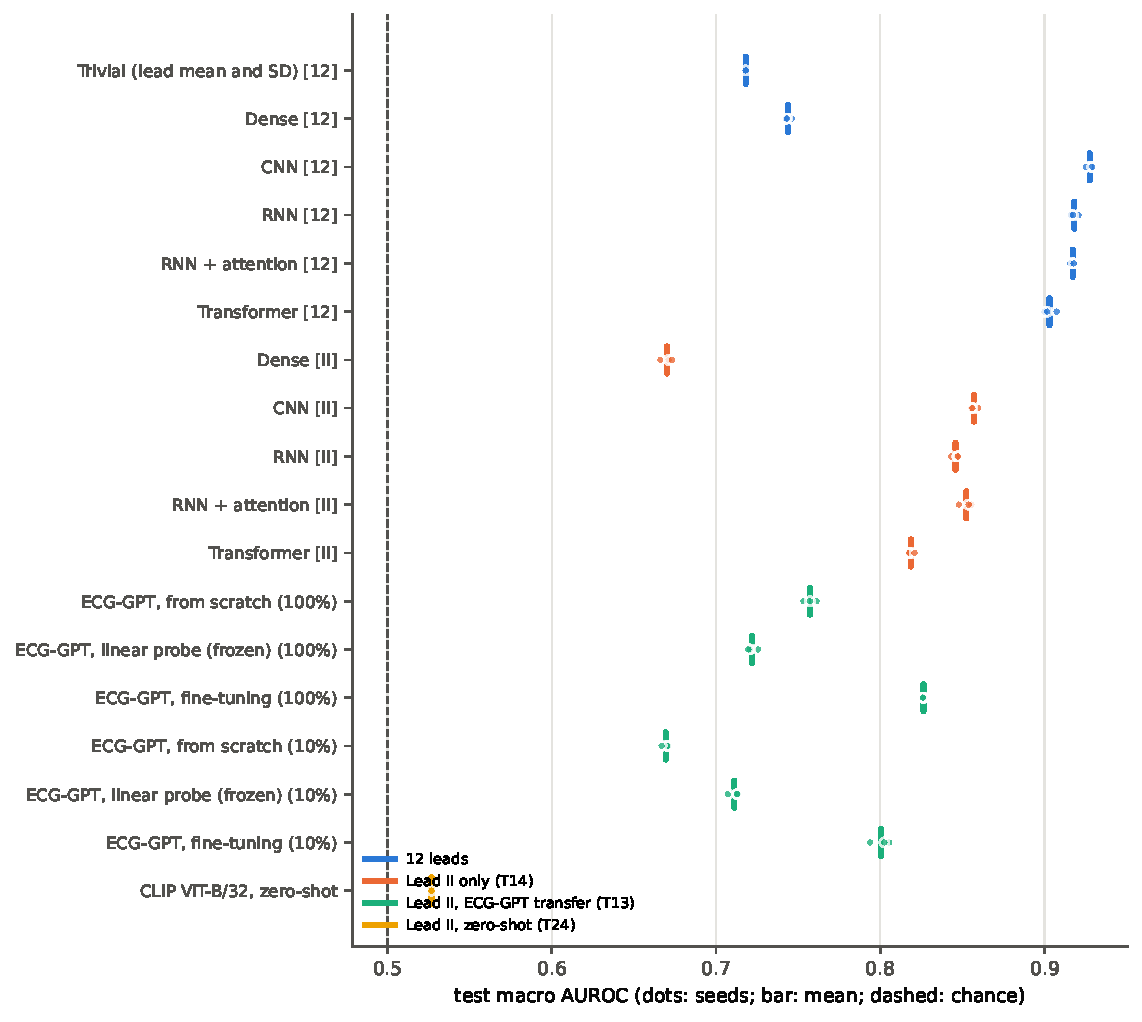
\includegraphics[width=\textwidth,height=0.42\textheight,keepaspectratio]{figures/comparison_overview.pdf}
\caption[All final models on the test fold]{Every final model on the test fold: macro AUROC (dots: seeds; bar: mean; dashed: chance). Blue: 12 leads; orange: lead II; green: ECG-GPT transfer (lead II); yellow: zero-shot CLIP (lead II images).}
\label{fig:comparison_overview}
\end{figure}


\subsection{Comparison with published results}

The last rows of Table~\ref{tab:comparison_final} are the eight models of the superclass column of
Table~I of the PTB-XL benchmark \cite{strodthoff2021deep}, the only numbers of the project typed by hand,
each stored with its file, page and quote. They share our task, our folds (training 1--8, validation 9,
test 10), our sampling rate and our metric, and they also leave out the records without a superclass
\cite{strodthoff2021deep}. But the setting is different in ways that matter, and the values are not
adjusted:
\begin{itemize}[leftmargin=1.2em,itemsep=1pt]
  \item they train on windows of 2.5\,s and aggregate the predictions over windows ``using the
        element-wise maximum'' \cite{strodthoff2021deep}, while our models see the whole 10\,s record;
  \item they use the AdamW optimiser with a 1-cycle learning-rate schedule \cite{strodthoff2021deep};
        we use Adam with a fixed rate;
  \item each published value is one trained model evaluated on the whole test set, with an interval given
        as the maximal deviation of the bootstrap bounds \cite{strodthoff2021deep}; ours are means over
        three seeds, with patient-bootstrap intervals for the first seed.
\end{itemize}
With those caveats, our CNN (\comparisonTestAurocMeanTwelveCnn{}) and the published residual network
(\comparisonPublishedStrodthoffResnetOneDWang{}) are in the same range, and our final RNN
(\comparisonTestAurocMeanTwelveRnn{}) is slightly below the published LSTMs
(\comparisonPublishedStrodthoffLstm{} and \comparisonPublishedStrodthoffLstmBidir{}). The conclusion I draw is modest: our small models, trained
within a course and a 4\,GB GPU, behave like the published baselines of the same families. They are not
meant to compete with them, which the guidelines explicitly do not ask for \cite{course_message_2011}.

% Shared float (common/make_floats.py). Table: tables/comparison_per_class.tex
\begin{table}[htbp]
\centering
\caption[Test AUROC per superclass]{Test AUROC per superclass of every final model (mean over seeds).}
\label{tab:comparison_per_class}
\small
\begin{adjustbox}{max width=\textwidth}
% Generated by src/comparison.py: test AUROC per superclass, mean over seeds.
\begin{tabular}{lccccc}
\toprule
Model & NORM & MI & STTC & CD & HYP \\
\midrule
\multicolumn{6}{l}{\textit{12 leads}} \\
\quad Trivial (lead mean and SD) & \comparisonTestAurocNORMMeanTrivial{} & \comparisonTestAurocMIMeanTrivial{} & \comparisonTestAurocSTTCMeanTrivial{} & \comparisonTestAurocCDMeanTrivial{} & \comparisonTestAurocHYPMeanTrivial{} \\
\quad Dense & \comparisonTestAurocNORMMeanTwelveDense{} & \comparisonTestAurocMIMeanTwelveDense{} & \comparisonTestAurocSTTCMeanTwelveDense{} & \comparisonTestAurocCDMeanTwelveDense{} & \comparisonTestAurocHYPMeanTwelveDense{} \\
\quad CNN & \comparisonTestAurocNORMMeanTwelveCnn{} & \comparisonTestAurocMIMeanTwelveCnn{} & \comparisonTestAurocSTTCMeanTwelveCnn{} & \comparisonTestAurocCDMeanTwelveCnn{} & \comparisonTestAurocHYPMeanTwelveCnn{} \\
\quad RNN & \comparisonTestAurocNORMMeanTwelveRnn{} & \comparisonTestAurocMIMeanTwelveRnn{} & \comparisonTestAurocSTTCMeanTwelveRnn{} & \comparisonTestAurocCDMeanTwelveRnn{} & \comparisonTestAurocHYPMeanTwelveRnn{} \\
\quad RNN + attention & \comparisonTestAurocNORMMeanTwelveRnnattn{} & \comparisonTestAurocMIMeanTwelveRnnattn{} & \comparisonTestAurocSTTCMeanTwelveRnnattn{} & \comparisonTestAurocCDMeanTwelveRnnattn{} & \comparisonTestAurocHYPMeanTwelveRnnattn{} \\
\quad Transformer & \comparisonTestAurocNORMMeanTwelveTransformer{} & \comparisonTestAurocMIMeanTwelveTransformer{} & \comparisonTestAurocSTTCMeanTwelveTransformer{} & \comparisonTestAurocCDMeanTwelveTransformer{} & \comparisonTestAurocHYPMeanTwelveTransformer{} \\
\multicolumn{6}{l}{\textit{Lead II only (T14)}} \\
\quad Dense & \comparisonTestAurocNORMMeanOneleadDense{} & \comparisonTestAurocMIMeanOneleadDense{} & \comparisonTestAurocSTTCMeanOneleadDense{} & \comparisonTestAurocCDMeanOneleadDense{} & \comparisonTestAurocHYPMeanOneleadDense{} \\
\quad CNN & \comparisonTestAurocNORMMeanOneleadCnn{} & \comparisonTestAurocMIMeanOneleadCnn{} & \comparisonTestAurocSTTCMeanOneleadCnn{} & \comparisonTestAurocCDMeanOneleadCnn{} & \comparisonTestAurocHYPMeanOneleadCnn{} \\
\quad RNN & \comparisonTestAurocNORMMeanOneleadRnn{} & \comparisonTestAurocMIMeanOneleadRnn{} & \comparisonTestAurocSTTCMeanOneleadRnn{} & \comparisonTestAurocCDMeanOneleadRnn{} & \comparisonTestAurocHYPMeanOneleadRnn{} \\
\quad RNN + attention & \comparisonTestAurocNORMMeanOneleadRnnattn{} & \comparisonTestAurocMIMeanOneleadRnnattn{} & \comparisonTestAurocSTTCMeanOneleadRnnattn{} & \comparisonTestAurocCDMeanOneleadRnnattn{} & \comparisonTestAurocHYPMeanOneleadRnnattn{} \\
\quad Transformer & \comparisonTestAurocNORMMeanOneleadTransformer{} & \comparisonTestAurocMIMeanOneleadTransformer{} & \comparisonTestAurocSTTCMeanOneleadTransformer{} & \comparisonTestAurocCDMeanOneleadTransformer{} & \comparisonTestAurocHYPMeanOneleadTransformer{} \\
\multicolumn{6}{l}{\textit{Lead II, ECG-GPT transfer (T13)}} \\
\quad ECG-GPT, from scratch, 100\% & \comparisonTestAurocNORMMeanScratchFOneZeroZero{} & \comparisonTestAurocMIMeanScratchFOneZeroZero{} & \comparisonTestAurocSTTCMeanScratchFOneZeroZero{} & \comparisonTestAurocCDMeanScratchFOneZeroZero{} & \comparisonTestAurocHYPMeanScratchFOneZeroZero{} \\
\quad ECG-GPT, linear probe (frozen), 100\% & \comparisonTestAurocNORMMeanProbeFOneZeroZero{} & \comparisonTestAurocMIMeanProbeFOneZeroZero{} & \comparisonTestAurocSTTCMeanProbeFOneZeroZero{} & \comparisonTestAurocCDMeanProbeFOneZeroZero{} & \comparisonTestAurocHYPMeanProbeFOneZeroZero{} \\
\quad ECG-GPT, fine-tuning, 100\% & \comparisonTestAurocNORMMeanFinetuneFOneZeroZero{} & \comparisonTestAurocMIMeanFinetuneFOneZeroZero{} & \comparisonTestAurocSTTCMeanFinetuneFOneZeroZero{} & \comparisonTestAurocCDMeanFinetuneFOneZeroZero{} & \comparisonTestAurocHYPMeanFinetuneFOneZeroZero{} \\
\quad ECG-GPT, from scratch, 10\% & \comparisonTestAurocNORMMeanScratchFOneZero{} & \comparisonTestAurocMIMeanScratchFOneZero{} & \comparisonTestAurocSTTCMeanScratchFOneZero{} & \comparisonTestAurocCDMeanScratchFOneZero{} & \comparisonTestAurocHYPMeanScratchFOneZero{} \\
\quad ECG-GPT, linear probe (frozen), 10\% & \comparisonTestAurocNORMMeanProbeFOneZero{} & \comparisonTestAurocMIMeanProbeFOneZero{} & \comparisonTestAurocSTTCMeanProbeFOneZero{} & \comparisonTestAurocCDMeanProbeFOneZero{} & \comparisonTestAurocHYPMeanProbeFOneZero{} \\
\quad ECG-GPT, fine-tuning, 10\% & \comparisonTestAurocNORMMeanFinetuneFOneZero{} & \comparisonTestAurocMIMeanFinetuneFOneZero{} & \comparisonTestAurocSTTCMeanFinetuneFOneZero{} & \comparisonTestAurocCDMeanFinetuneFOneZero{} & \comparisonTestAurocHYPMeanFinetuneFOneZero{} \\
\multicolumn{6}{l}{\textit{Lead II, zero-shot (T24)}} \\
\quad CLIP ViT-B/32, zero-shot & \comparisonTestAurocNORMMeanZeroshot{} & \comparisonTestAurocMIMeanZeroshot{} & \comparisonTestAurocSTTCMeanZeroshot{} & \comparisonTestAurocCDMeanZeroshot{} & \comparisonTestAurocHYPMeanZeroshot{} \\
\bottomrule
\end{tabular}

\end{adjustbox}
\end{table}


\subsection{Limitations}

\begin{itemize}[leftmargin=1.2em,itemsep=1pt]
  \item \textbf{One dataset, one task, small budgets.} Every conclusion is about five superclasses of
        PTB-XL; long memory or the order of events may matter for other labels (rhythm, for example),
        which we did not test.
  \item \textbf{Three seeds.} They allow paired, per-seed statements, but the standard deviations over
        seeds rest on three values.
  \item \textbf{Selection rules fixed in advance.} They protect the test fold, but they can select a
        configuration only marginally different from its neighbours (the two final recurrent models, or
        \texttt{no\_pos} and \texttt{patch5} in the Transformer).
  \item \textbf{Interpretation figures.} Attention weights, attention maps and input sensitivities were
        computed for one seed and a few example records; what they show about QRS complexes is a visual
        observation, not a measured result.
  \item \textbf{Area 2.} The pre-trained model is small and pre-trained on PTB-XL itself, and zero-shot
        was tested with one general image--text model and fixed sentences.
\end{itemize}

\subsection{Conclusions}

\begin{enumerate}[leftmargin=1.4em,itemsep=2pt]
  \item \textbf{Weight sharing over time is the main ingredient.} All architectures that apply the same
        weights along the record (CNN, LSTM and GRU, attention models) are far above the dense network; the
        differences among them are small.
  \item \textbf{For recurrent networks, reading all hidden states matters more than the cell or the
        direction}, and a GRU was better than an LSTM. Attention pooling helped exactly as much as a mean
        and spread its weights almost uniformly: on this task it worked as a learned mean.
  \item \textbf{Self-attention is built from parts that each add something}, with the largest gains from
        several heads and from the residual path with LayerNorm. But no Transformer used the order of the
        patches, and the final one has no positional encoding: it classifies a set of beat fragments.
  \item \textbf{Local features win.} The best recurrent model has a convolutional front end, raw samples
        beat flattened frames, short patches beat long ones, and the CNN is the best model on 12 leads and
        on lead II, also against a fine-tuned self-supervised Transformer.
  \item \textbf{Methodology.} Deciding the protocol before the runs, pairing comparisons on the same
        patients and seeds, and generating every number from the logs made it possible to say which
        differences are real; several ablations change nothing in any seed, and the two final recurrent
        models cannot be told apart, and we report them so.
\end{enumerate}
